

	

\chapter{Chapitre 3}
\newpage
	\section{Introduction}
	
	Dans ce chapitre nous présenterons les différentes étapes de réalisation de notre projet. Nous avons choisi de construire notre montage à base d’un contrôleur de vol Apm 2.8 pour ses fonctionnalités. Notre drone est réalisé à l’aide de 4 moteurs qui sont commandés depuis ce contrôleur de vol  à travers des contrôleurs de vitesse électronique (ESC). L'ensemble de ces composants  est alimenté par une batterie et piloté à l’aide d’une radiocommande.
	\section{Matériels utilisés}
	Lors de notre réalisation, nous avons utilisé plusieurs composants que nous présentons ci-dessous.
	\subsection{Châssis}
	Le châssis représente le corps principal de notre quadrirotor. Il comprend quatre bras de forme ’X’. Ses caractéristiques à prendre en compte sont le poids, qui est lié aux matériaux utilisés et sa résistance au choc, plus le châssis est léger, plus nous conservons de la puissance.
	
	Pour éliminer les vibrations du moteur et pour obtenir les meilleures performances sur le côté aérodynamique, nous avons choisis d’utiliser un châssis professionnel "le DJI F450". Son assemblage est simple et rapide. Les 4 bras sont vissés entre la plaque inférieure et la plaque supérieure. Notre châssis a une envergure de 450 mm et pèse 272 grammes.
	Cette structure permet d’accueillir toute l’électronique : ESCs, moteurs, contrôleur de vol. En plus, Nous pouvons grâce au PCB intégré dans la plaque inférieure souder les pôles  du contrôleur de vitesse (+/-) et la batterie. La propulsion recommandée repose sur des moteurs 2212!!!!!!, des hélices 10x45 en 3S et 8x45 en 4S pour un poids total en vol situé entre 800 et 1600 grammes maximum.
	
	\begin{figure} [h]
		\begin{center}
			\centering
			\fbox{\includegraphics[width=0.3\linewidth]{Images/Châssis DJI F450}}
		\end{center}
		\caption{Châssis DJI F450}
	\end{figure}
	\newpage
	\subsection{Moteurs Brushless}
	Notre drone nécessite l'utilisation de moteurs ayant une très grande vitesse en considérant leur poids qui doit être léger. Ceci nous oblige d'utiliser des moteurs brushless 2212 (22 pour le diamètre et 12 pour l'hauteur) qui sont des moteurs à courant continu, n’utilisent pas de balais collecteurs car les bobines sont alimentées directement au stator et que les aimants sont placés sur le rotor[9]. Afin d'obtenir un vol stable et un couple de moteurs important, nous avons choisi ces composants possèdant 930KV. A savoir, KV représente la constante de vitesse qui est le nombre de tours par minutes divisé par les volts KV=RPM/U. Par exemple, lorsque nous attribuons à un moteur une tension de 10V, celui-ci tournera à 9300 tr/min. 
	\begin{figure} [h]
		\begin{center}
			\centering
			\fbox{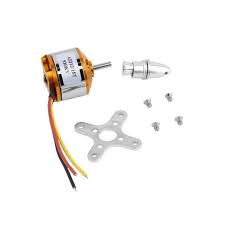
\includegraphics[width=0.3\linewidth]{Images/Moteur Brushless}}
		\end{center}
		\caption{Moteur Brushless}
	\end{figure}
	\subsection{Contrôleurs de vitesse électronique (ESC)}
	Concernant l'étage de puissance, nous avons opté pour un variateur de vitesse ESC (Electronic Speed Controller) pour contrôller l'énergie délivrée aux moteurs brushless  grâce à la tension de sortie modulable d’une carte programmable.  Ces appareils reçoivent des signaux PWM (Pulse Modulation Width) ou PPM (pulse position modulation). Vu que le variateur de vitesse doit être supérieur au courant maximum du moteur qui est de 10A, nous avons choisi un courant de 30A. 
	\par
	\begin{figure} [h]
		\begin{center}
			\centering
			\fbox{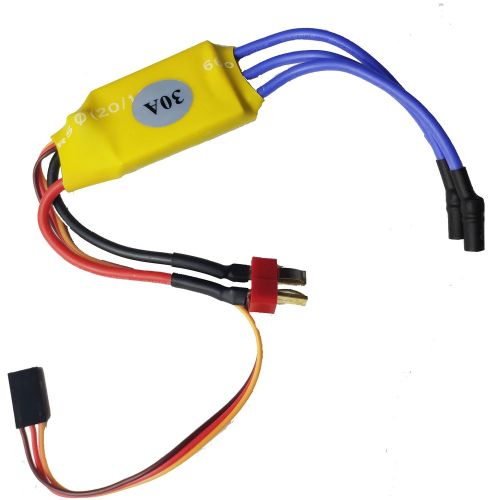
\includegraphics[width=0.3\linewidth]{Images/Contrôleur de vitesse électronique (ESC)}}
		\end{center}
		\caption{Contrôleur de vitesse électronique (ESC)}
	\end{figure}
	\newpage
	\subsection{Batterie}
	L'alimentation électrique de notre système est une procédure très importante pour le fonctionnement de notre quadrirotor. Pour cela, nous avons choisi d'utiliser une batterie LiPo (Lithium Polymère) puisqu'elle fournit suffisament de puissance pour une faible masse. Elle est fabriquée avec une technologie offrant un trés bon rapport poids/ puissance. Notre batterie est composée de 3 cellules, chacune possède une tension de 3.7V, c'est pour cette raison qu'elle délivre en total une tension de 11.1V. Conçernant son ampérage, elle fournit 3000 mA par heure.
	\par
	\begin{figure} [h]
		\begin{center}
			\centering
			\fbox{
\includegraphics[width=0.3\linewidth]{Images/Batterie Lipo 3S}}
		\end{center}
		\caption{Batterie Lipo 3S}
	\end{figure}
	\subsection{Hélice}
	L’hélice est un dispositif rotatif formé d’un certains nombre de pales ayant un profile d’aile. Le choix de ces composants est aussi important lors de la conception de notre drone dont il faut des hélices adaptées au type de vol que nous souhaitons réaliser. Puisque nous avons utilisé le châssis DJI F450 et la batterie Lipo 3s qui dépendent du choix des hélices, nous avons utilisé des pales 1045 ( 10 pour la longueur et 4.5 pour le pas).
	\begin{figure} [h]
		\begin{center}
			\centering
			\fbox{\includegraphics[width=0.3\linewidth]{Images/Hélice 1045}}
		\end{center}
		\caption{Hélice 1045}
	\end{figure}
	\subsection {Contrôleur de vol (APM 2.8)}[5]
	Le contrôleur de vol est l'élément central de l'électronique de notre drone.
	Nous avons sélectionné l’APM 2.8 comme étant un contrôleur de vol grâce à son système de pilotage automatique open source complet. Permettant aussi de contrôler plusieurs objets radiocommandes comme les avions, les voitures, les planeurs et les multirotors tel que hexarotor, trirotor et quadrirotor ...
	Ce contrôleur de vol constitue le cerveau de notre quadrirotor qui est capable d'effectuer des missions GPS programmées avec des points de cheminement. Il s’agit d’une carte microcontrôleur à puce ATMEGA328P!!! livrée avec un gyroscope, un accéléromètre, un magnétomètre et un baromètre intégrés à 3 axes!!!!.
	
	Dans notre cas, l’APM 2.8 est connecté avec le récepteur de la radiocommande dans les broches d’entrée ainsi qu'avec les contrôleurs de vitesse ESC dans les broches de sortie. 
	
	\begin{figure} [h]
		\begin{center}
			\centering
			\fbox{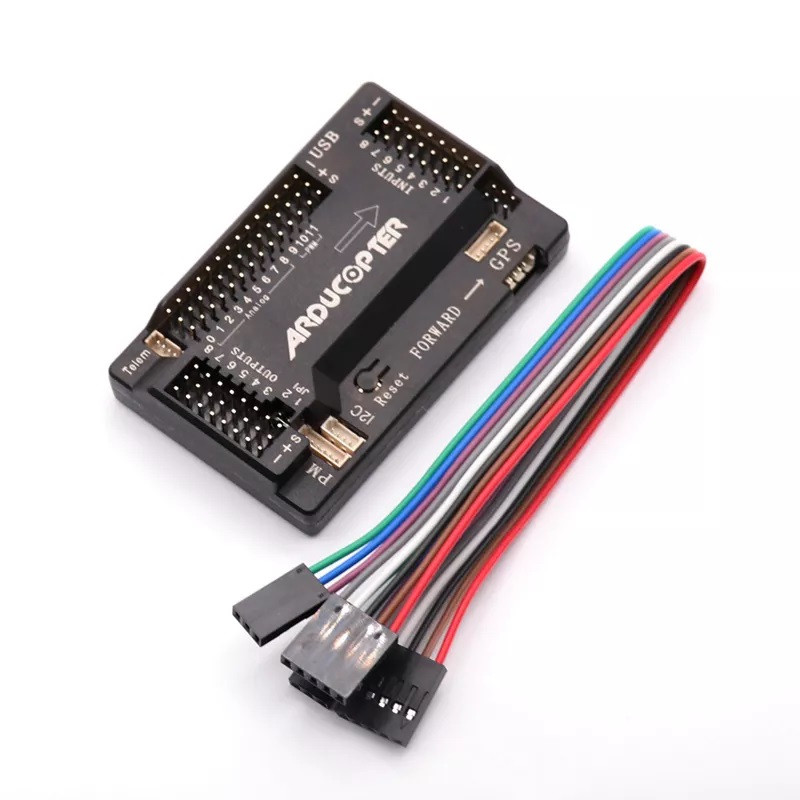
\includegraphics[width=0.3\linewidth]{Images/controlleur-de-vol-ardupilot-apm28}}
		\end{center}
		\caption{calibration du radio}
	\end{figure}
	\newpage
	\subsection {Radiocomamande}
	Une radiocommande est un outil permettant de contrôler à distance notre drone à travers des signaux radio. Nous avons choisi cet appareil grâce à sa portée et sa latence qui sont importantes par rapport au wifi et au bluetooth. Son émetteur est de type Turnigy 9x et son récepteur de type IA8 AFHDS2A.
	
	\subsubsection{Emetteur} 
	La Turnigy 9x est une radio de 9 voies, elle est équipée de 6 interrupteurs de deux positions, un interrupteur de trois position et de trois potentiomètres rotatifs.
	De plus, grâce à la technologie 2,4 Ghz, nous disposons d'une réaction ultra-rapide et d'un contrôle sans interférence. Pour la
	conception ergonomique, celle-ci facilite l'utilisation de toutes les commandes dont les interrupteurs et les ports sont tous positionnés pour plus de confort. En plus, les bâtons de longueur réglable peuvent être adaptés à nos besoins et l' écran LCD monochrome facilite la programmation ainsi que la modification des paramètres. 
	
	\begin{figure} [h]
		\begin{center}
			\centering
			\fbox{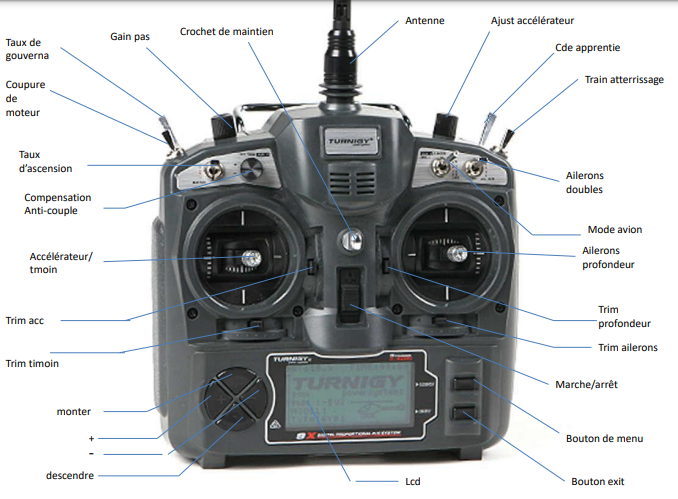
\includegraphics[width=0.8\textwidth]{Images/Emetteur radiocommande}}
		\end{center}
		\caption{calibration du radio}
	\end{figure}
	\subsubsection{Récepteur }
	Ce récepteur IA8 AFHDS 2A dispose de 8 voies et fonctionne parfaitement avec la radiocommande Turnigy 9x système AFHDS 2A. Il a une portée de plus de 500 mètres  grâce à ses deux antennes. En plus, Ce composant reste très compact et fonctionne en PWM!!!!!! ou PPM .
	\begin{figure} [h]
		\begin{center}
			\centering
			\fbox{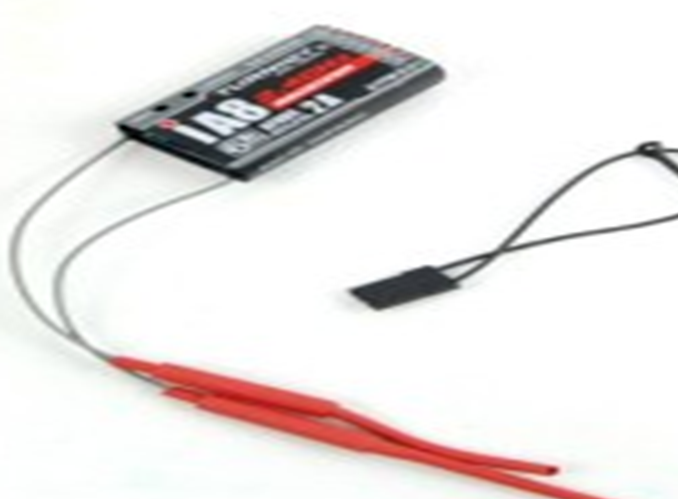
\includegraphics[width=0.4\textwidth]{Images/Récépteur radiocommande}}
		\end{center}
		\caption{calibration du radio}
	\end{figure}
	\subsection {Diodes  et résistances}
	Afin d'éclairer notre quadrirotor, nous avons utilisé 8 diodes ( 4 diodes blanches et 4  rouges) pour mieux connaître son mouvement. Nous avons utilisé 5v  de l'Apm 2.8. Puisqu'une diode a besoin de 3 v et 5 mA, nous avons choisi une résistance de \SI{330}{\ohm} à chaque diode pour encaisser les 2 v supplémentaires et tout cela sous 5 mA.
	\begin{figure}[h]
		\centering
		\begin{minipage}{0.49\textwidth}
			\fbox{\hspace*{1cm}\includegraphics[width=0.8\textwidth]{C:/Users/Ahmed Baha eddine/Downloads/Led(blanc-rouge)}}
			\caption{Diodes}
			\label{fig:my_label1}
		\end{minipage}
		\begin{minipage}{0.49\textwidth}
			\fbox{\hspace*{1.2cm}\includegraphics[width=0.8\textwidth]{C:/Users/Ahmed Baha eddine/Downloads/resistance4}}
			\caption{Résistance}
			\label{fig:my_label}
		\end{minipage}
	\end{figure}
	\section{Logiciels utilisés}
	Dans notre projet, nous avons travaillé sur de nombreux logiciels que nous traitons un par un.
	\subsubsection{Latex}
	Nous avons choisi comme éditeur de texte le logiciel Latex car il nous  offre de nombreuses fonctionnalités et nous permet de composer une très grande variété de formules mathématiques.
	\begin{figure}[h]
		\begin{center}
			\centering
			\fbox{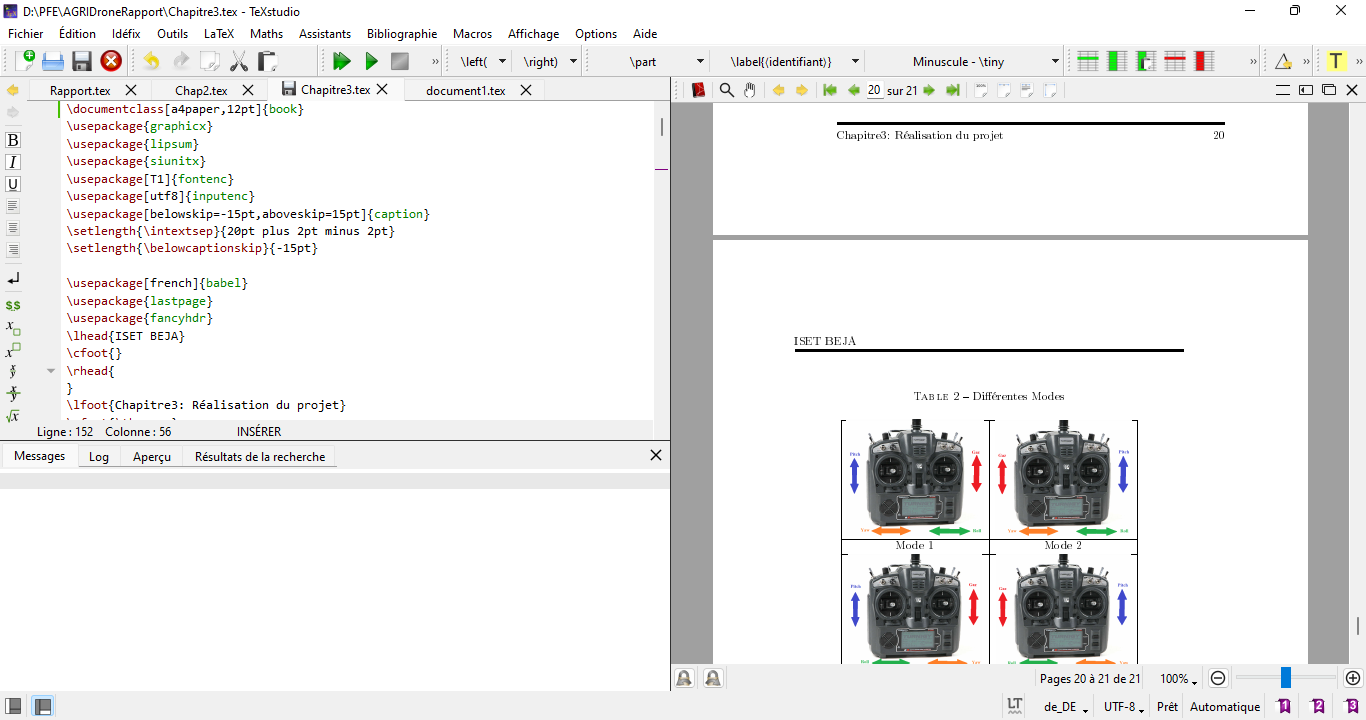
\includegraphics[width=0.6\linewidth]{Images/Latex}}
		\end{center}
		\caption{Les 4 modes}
	\end{figure}
	\subsubsection{Google Drive}
	Dans le but de partager et de collaborer notre travail, nous avons utlilisé google drive qui nous permet de travailler sur les différents documents à produire au cours du projet.
	\begin{figure}[h]
		\begin{center}
			\centering
			\fbox{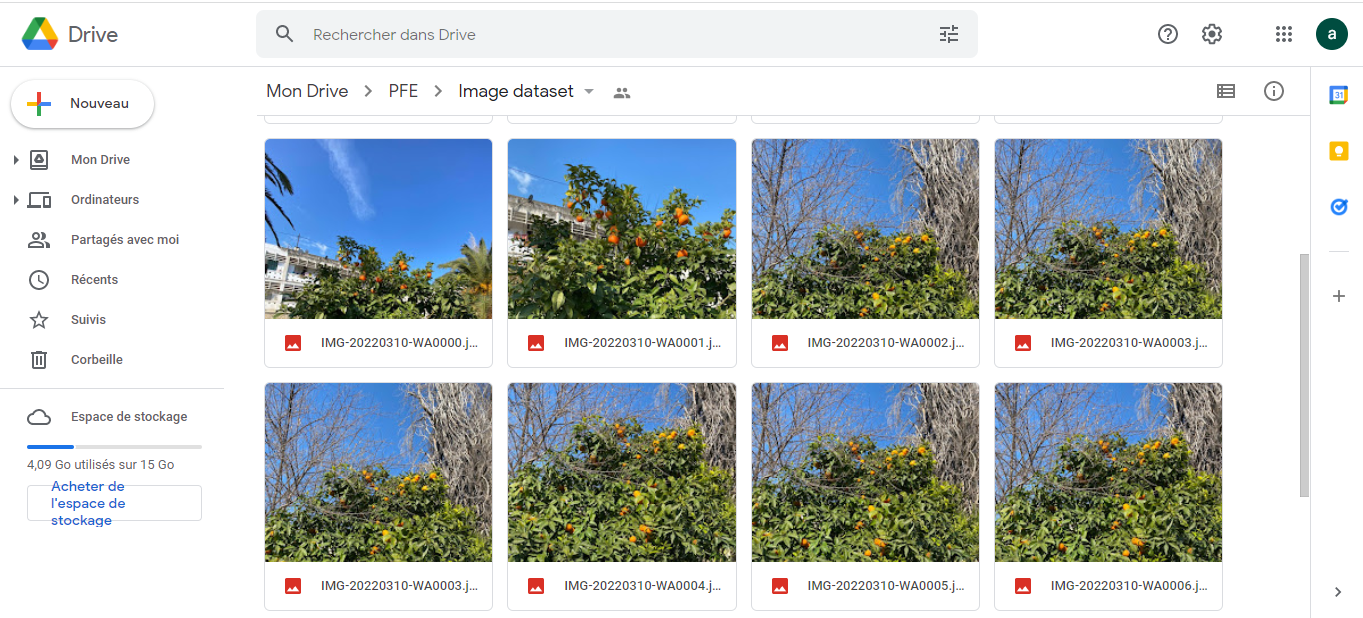
\includegraphics[width=0.6\linewidth]{Images/Google drive}}
		\end{center}
		\caption{Les 4 modes}
	\end{figure}
	\subsubsection{Jira Software}
	Nous avons sélectionné jira software comme étant un outil de gestion de notre projet puisqu'il est  puissant et nous permet de visualiser l'avancement de notre travail grâce aux tableaux Agile. En plus, il nous offre la possibilité de travailler à distance grâce à cette platforme.
	\begin{figure}[h]
		\begin{center}
			\centering
			\fbox{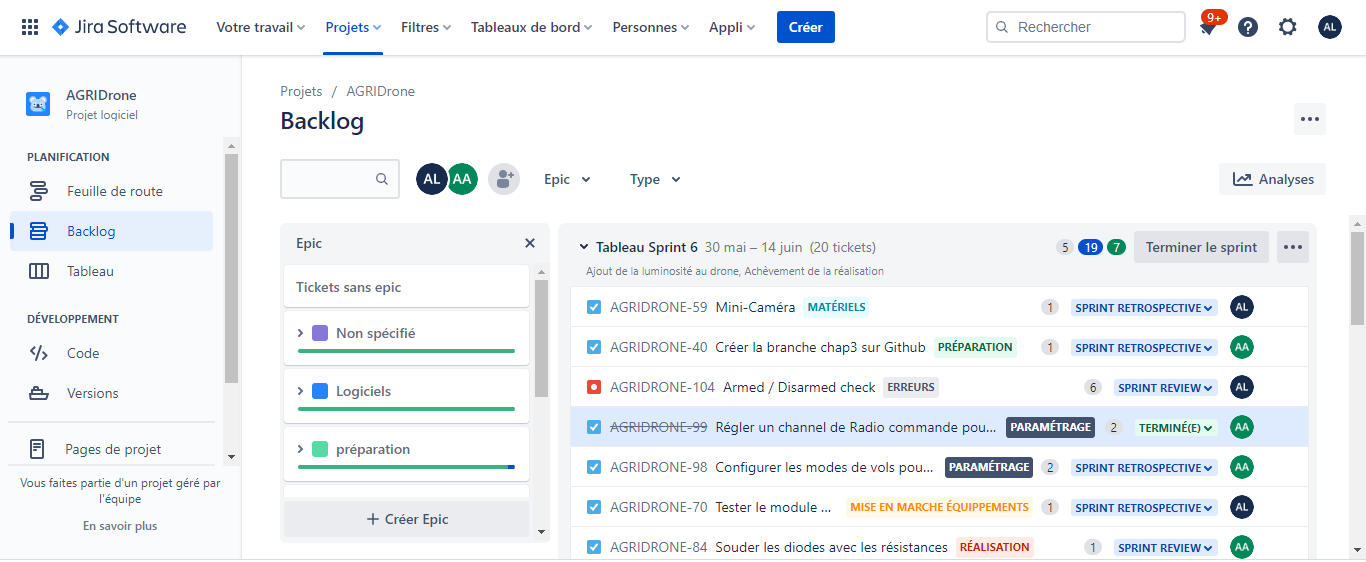
\includegraphics[width=0.6\linewidth]{Images/Jira}}
		\end{center}
		\caption{Les 4 modes}
	\end{figure}
	\subsubsection{Github}
	Github est utilisé pour la centralisation et la gestion du code source , des documets et des différents modules du projet. Ce service est utilisé puisque le projet se trouvait déjà sur cette plateforme et qu’elle est facile à utiliser.
	\begin{figure}[h]
		\begin{center}
			\centering
			\fbox{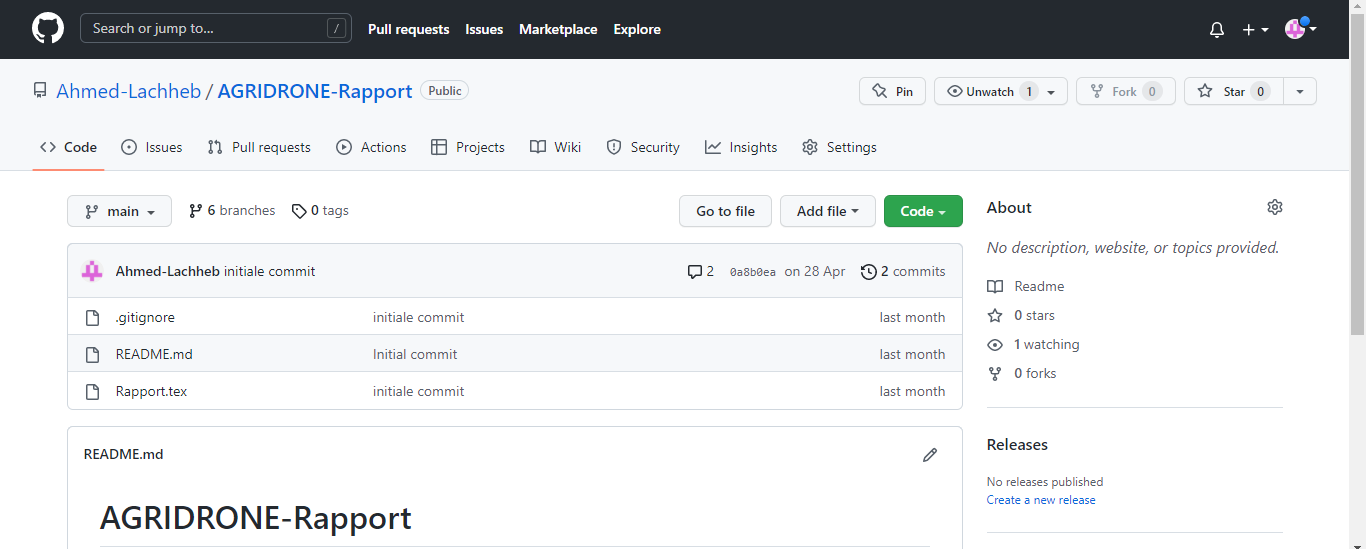
\includegraphics[width=0.7\linewidth]{Images/Github}}
		\end{center}
		\caption{Les 4 modes}
	\end{figure}
	\subsubsection{Papyrus}
	C'est un logiciel gratuit qui est riche en fonction dont il nous a aidé à faire la conception de notre projet à travers les diagrammes de cas d'utilisation.
	\begin{figure}[h]
		\begin{center}
			\centering
			\fbox{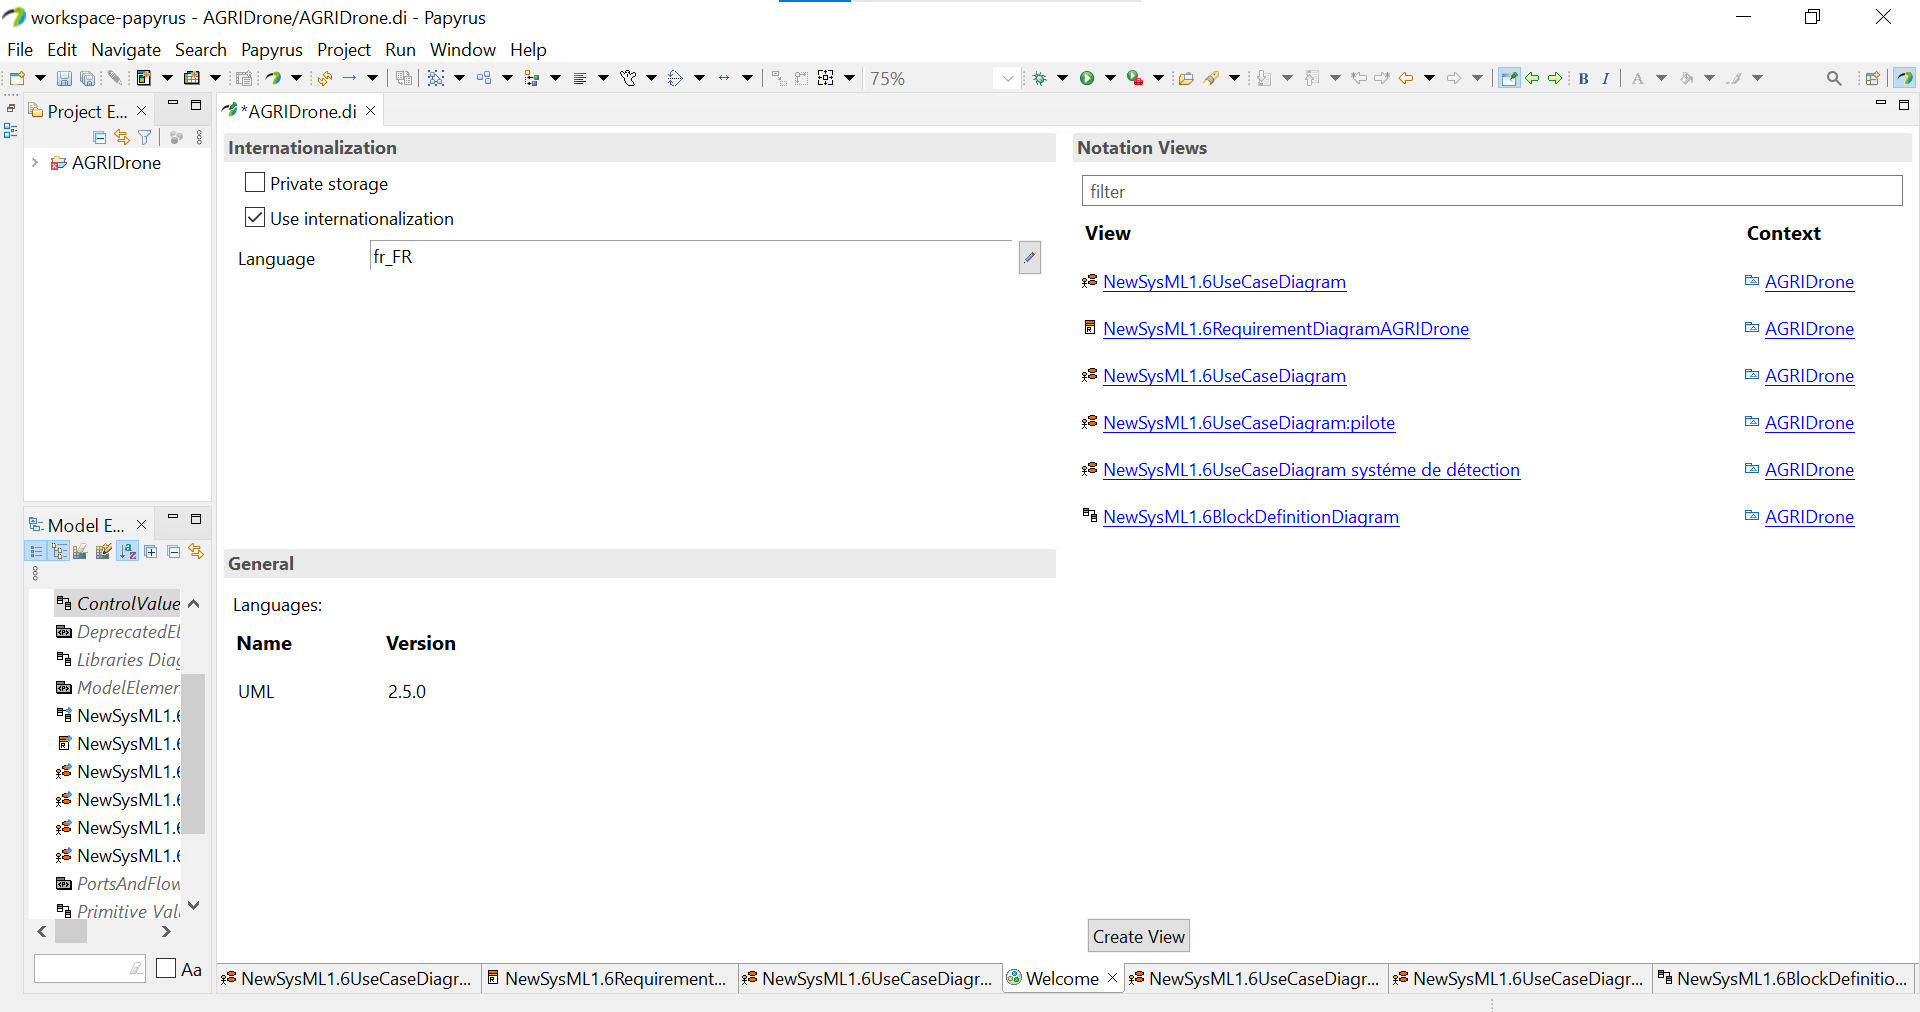
\includegraphics[width=0.6\linewidth]{Images/papyrus}}
		\end{center}
		\caption{Les 4 modes}
	\end{figure}
	\newpage
	\subsubsection{Visual Paradigm}
	Suite à des obstacles que nous avons rencontré au niveau de Papy-rus, nous avons recours à Visual Paradigm pour la réalisation des diagrammes d'exigence et de définition de bloc.
	\begin{figure}[h]
		\begin{center}
			\centering
			\fbox{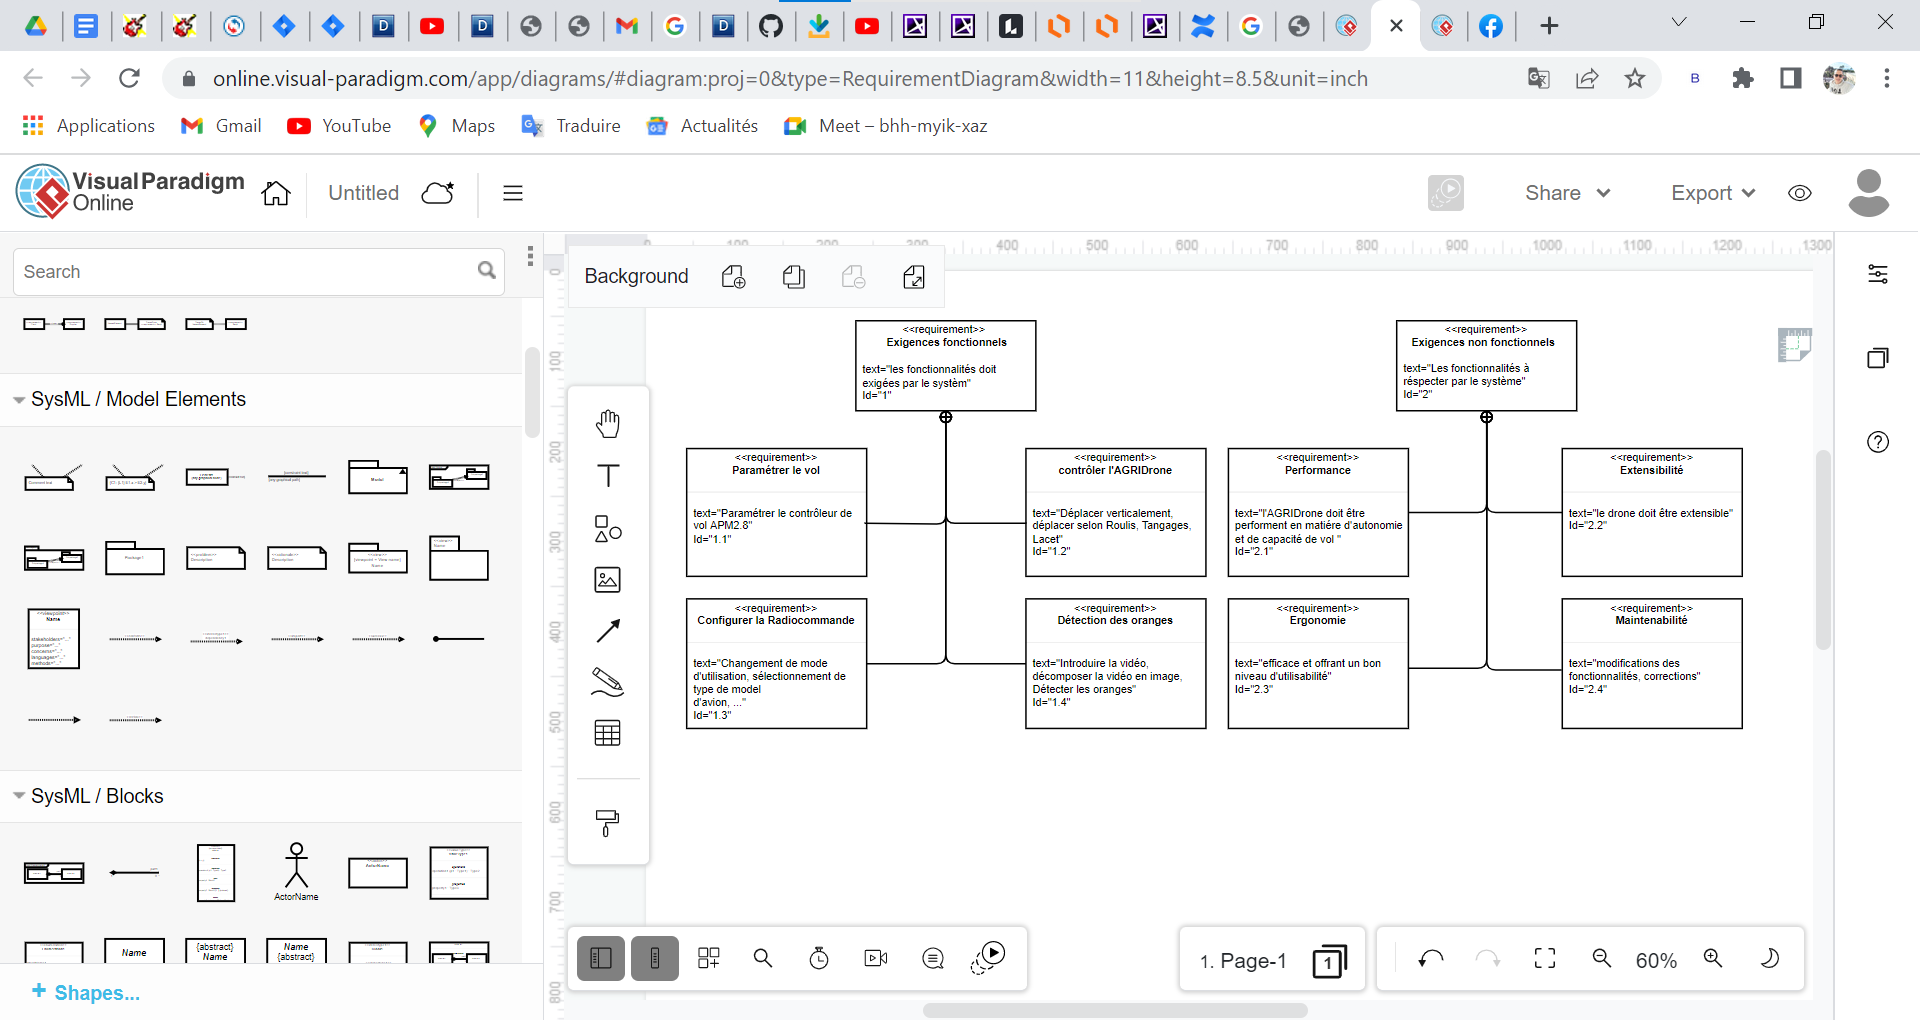
\includegraphics[width=0.6\linewidth]{Images/Visual Paradigm}}
		\end{center}
		\caption{Les 4 modes}
	\end{figure}
	\subsubsection{Companion 9x}
	Nous avons utilisé ce logiciel pour flacher la radiocommandele en téléversant le frimware via la mémoire de l'émetteur du radiocommande.
	\begin{figure}[h]
		\begin{center}
			\centering
			\fbox{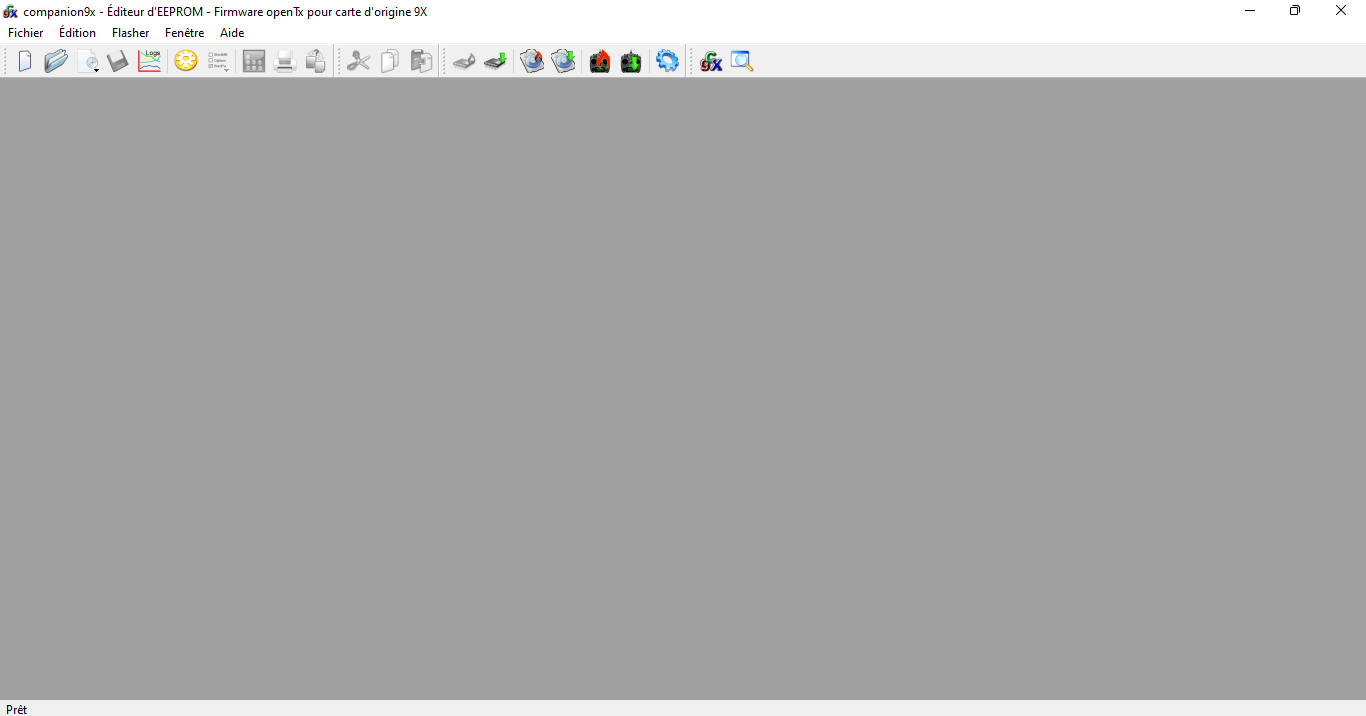
\includegraphics[width=0.6\linewidth]{Images/Companion 9x}}
		\end{center}
		\caption{Les 4 modes}
	\end{figure}
	\newpage
	\subsubsection{Jabref}
	JabRef est un logiciel que nous avons utilisé dans la gestion bibliographique. Il nous fournit une interface conviviale pour éditer des fichiers Bib(La)TeX.
	\begin{figure}[h]
		\begin{center}
			\centering
			\fbox{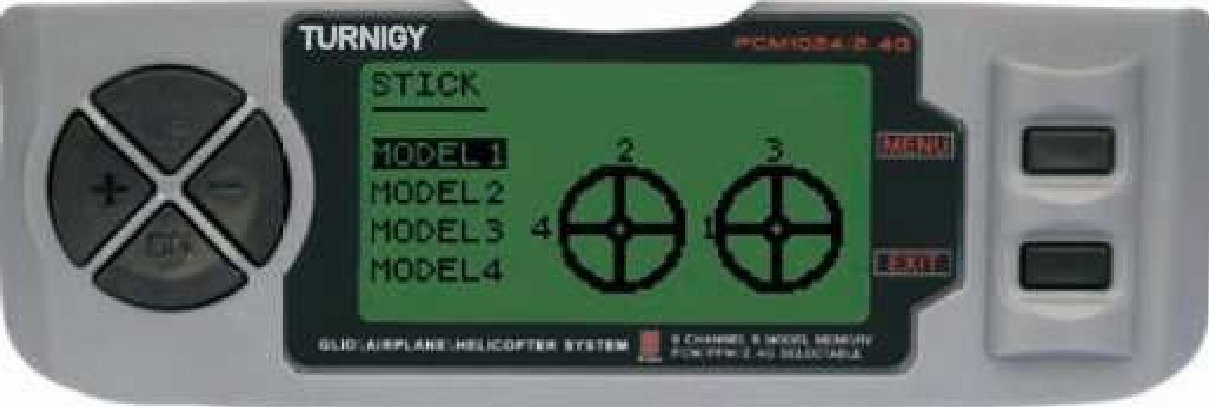
\includegraphics[width=0.6\linewidth]{Images/Les 4 modes}}
		\end{center}
		\caption{Les 4 modes}
	\end{figure}
	\subsection{Mission Planner	}
	Ce logiciel représente une station de contrôle au sol pour les hélicoptères, avions ou rovers. Il nous a permis de paramétrer notre contrôleur de vol et de configurer ses différents paramètres ainsi que d'assurer ses performances optimales.
	\begin{figure} [h]
		\begin{center}
			\centering
			\hspace*{1.5cm}\fbox{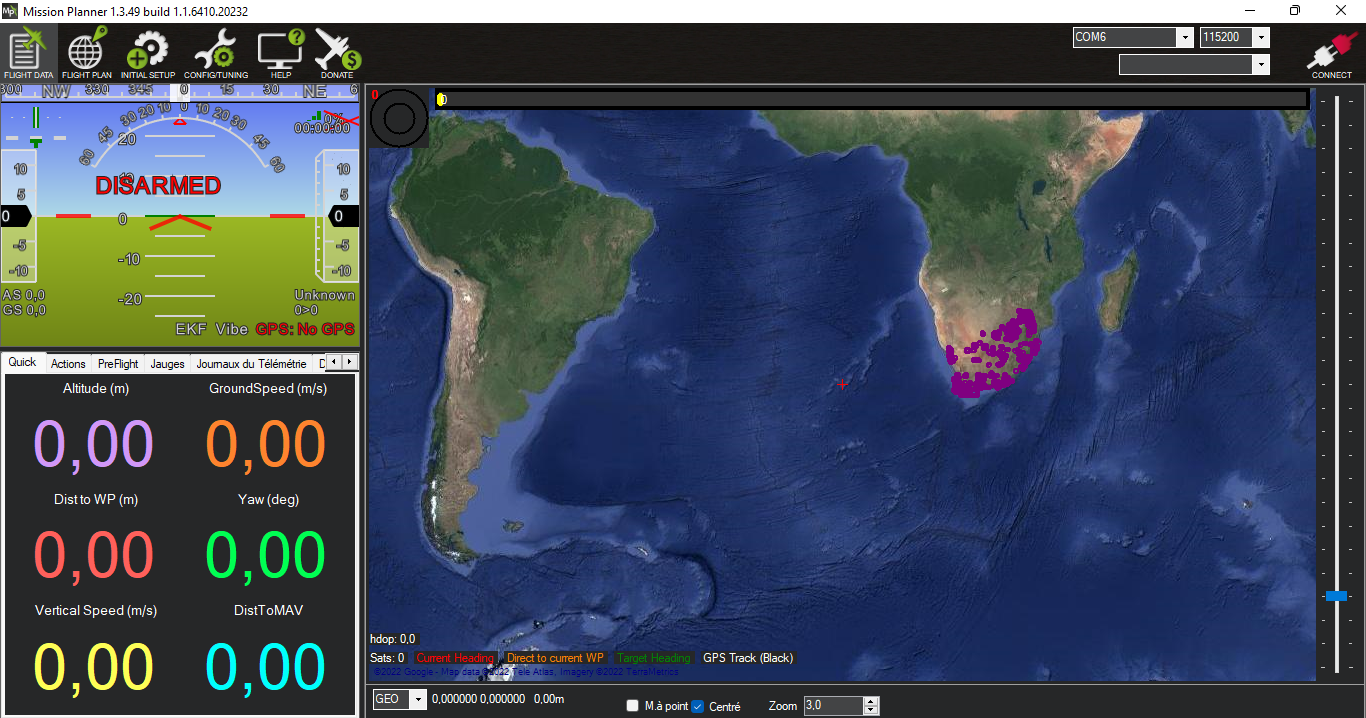
\includegraphics[width=0.7\linewidth]{Images/Interface de Mission Planner}}
			\centering
			\hspace*{1.5cm}	\caption{Interface de Mission Planner}
		\end{center}
	\end{figure}
	\newpage
	\section{Montage des composants}
	Pour réaliser notre drone on a poursuivi le schéma électrique présenté ci-dessous :
	
	\begin{figure} [h]
		\begin{center}
			\centering
			\hspace*{-1cm}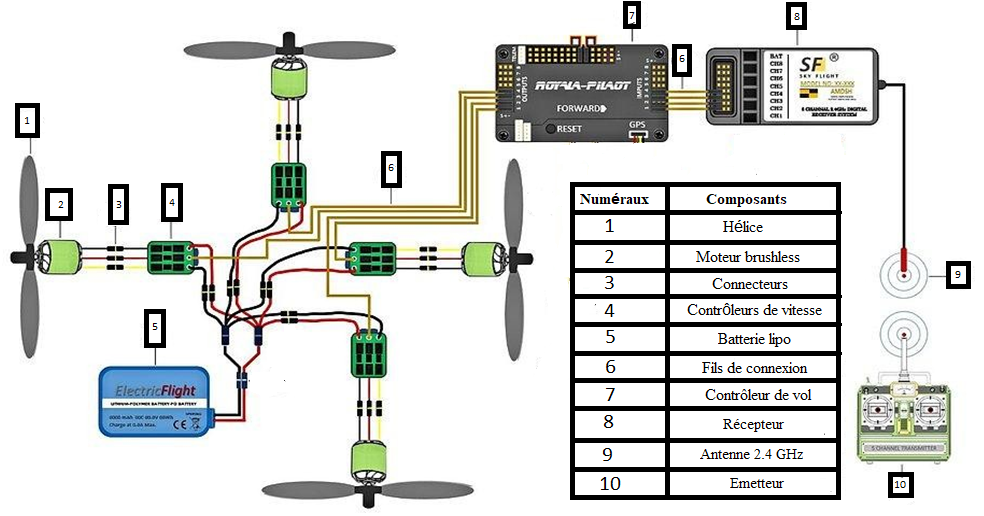
\includegraphics[width=1.1\linewidth]{Images/Shéma électrique}
		\end{center}
		\caption{Montage des composant}
	\end{figure}
	
	
	\section{Configurations et calibrations}
	Puisque le contrôleur de vol et la radiocommande fonctionnent sur différents modèles d'avions, il est nécessaire de leurs effectuer des configurations  ainsi que  des calibrations spécifiques pour le fonctionnement de notre quadrirotor. 
	\subsection{Configurations et calibrations de l'APM 2.8}
	Pour configurer et calibrer l'APM 2.8, il nous reste  de lancer l’assistant et le connecter en USB sur notre PC.
	\subsubsection{Chargement du firmware }
	Ensuite, nous avons accédé au menu "INITIAL SETUP". L'installation du frimware se fait en cliquant sur le bouton "Install Frimware". Cette opération commence après avoir séléctionné le type du multicoptère, dans notre cas c'est le "quadrirotor" que nous avons chargé.  la dernière version du firmware dans
	notre carte APM2.8 est présenté dans la figure ci-dessous . Le logo "CONNECT" doit rester rouge c'est à dire en mode déconnecté. Dès que le frimware est installé, le drone sera prêt à être configuré et paramétré.
	\begin{figure}[h]
		\begin{center}
			\centering
			\fbox{ 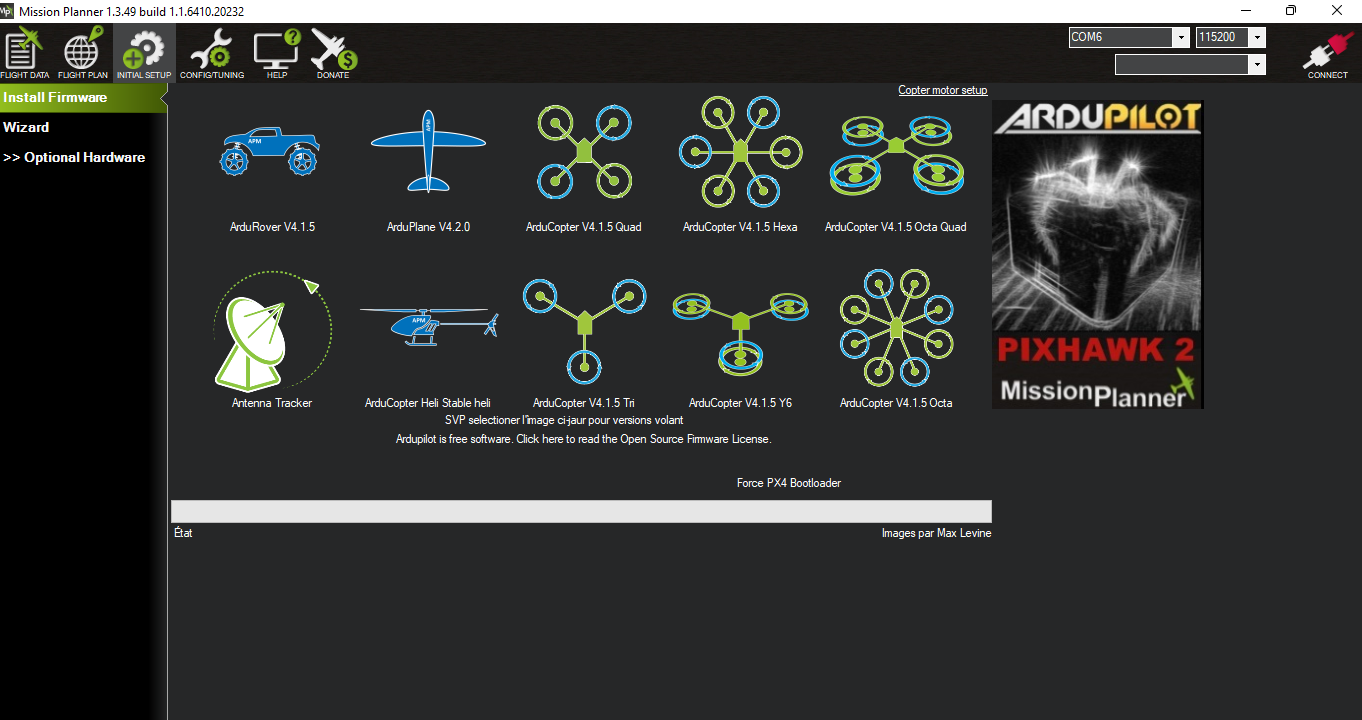
\includegraphics[width=0.6\linewidth]{Images/Chargement du firmware}}
		\end{center}
		\caption{Les 4 modes}
	\end{figure}
	
	\subsubsection{Type de Châssis}
	Après avoir installé le frimware, nous avons connecté  la carte APM 2.8 en haut à droite de Mission Planner. Pour s'assurer que la carte Apm est bien connectée, le logo "CONNECT" doit passer de la couleur rouge à la couleur verte. Ensuite, nous avons cliqué sur "INITIAL SETUP", "Mandatory Hardware" et "Frame Type" afin de  configurer le type de notre quadrirotor. 
	\begin{figure}[h]
		\begin{center}
			\centering
			\fbox{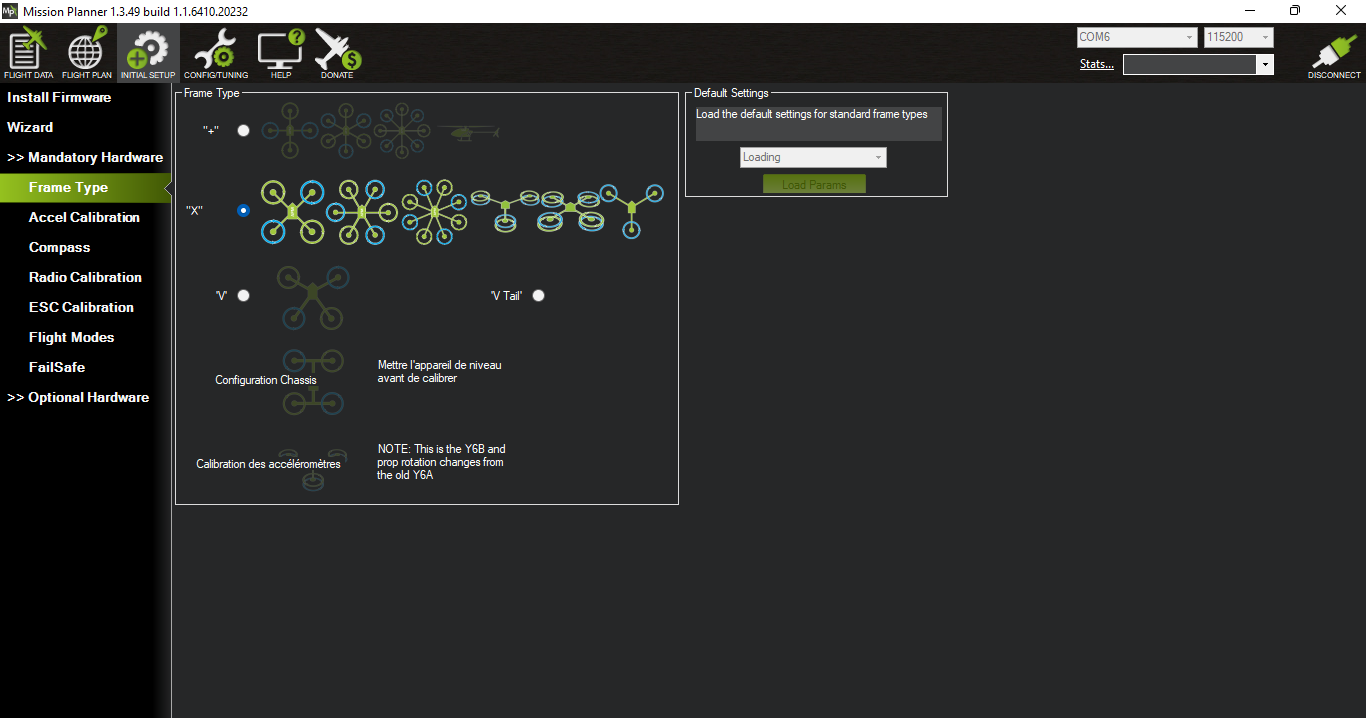
\includegraphics[width=0.6\linewidth]{Images/Choix du type de quadrirotor}}
		\end{center}
		\caption{calibration du magnétométre}
	\end{figure}
	\subsection{Calibration du magnétomètre}
	Pour réaliser cette manipulation, il est préférable de connecter le contrôleur de vol avec un câble USB afin d’obtenir un échantillonnage précis et continu.
	Dans la sous-section « Compass », il vaut mieux vérifier que le magnétomètre est activé ainsi que la déclinaison soit automatique.
	
	\begin{figure}[h]
		\begin{center}
			\centering
			\fbox{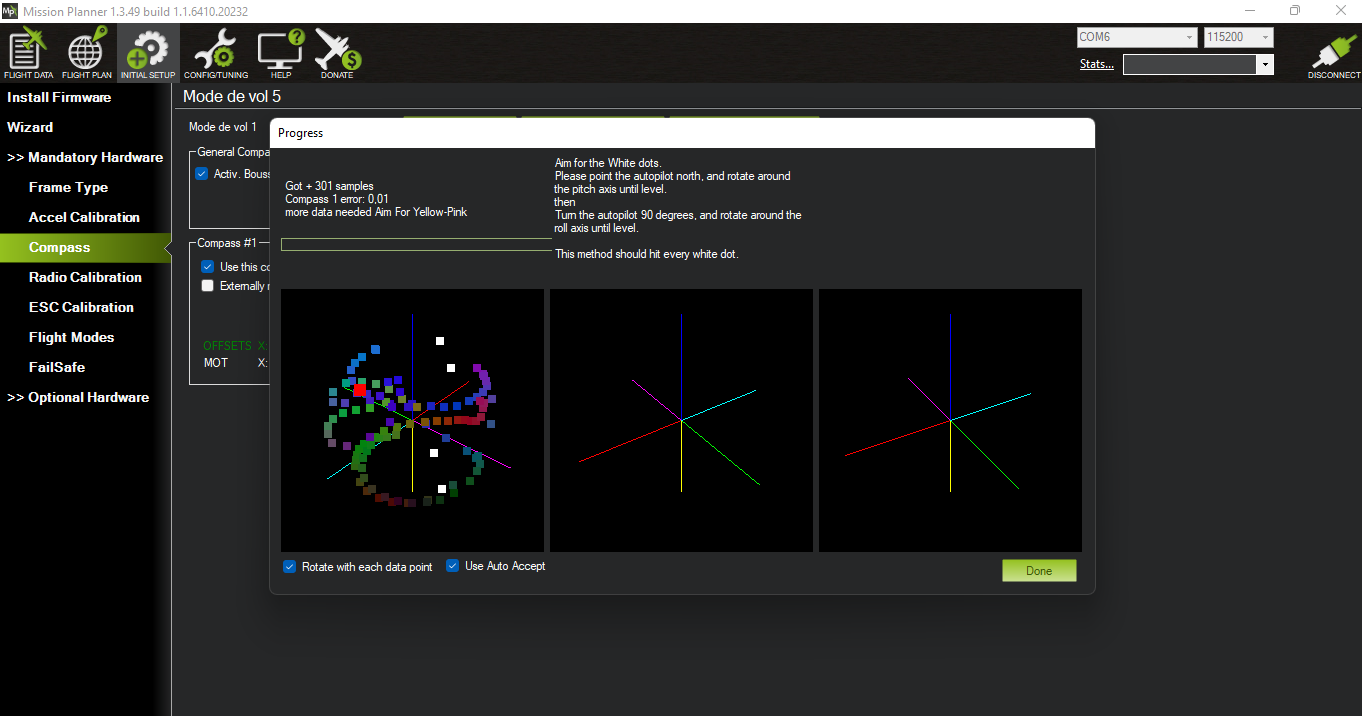
\includegraphics[width=0.6\linewidth]{Images/calibration du magnétométre}}
		\end{center}
		\caption{calibration du magnétométre}
	\end{figure}
	
	\subsection{Calibration des accéléromètres}
	Pour un résultat optimal,  premiérement nous devons accéder au menu "INITIAL SETUP", deuxiément "Mandatory Hardware" et finalement, "Accel Calibration". L'APM2.8 doit être positionnée successivement sur chacune de ses six faces.
	La séquence se présente de la façon suivante :
	\begin{table}[H]
		\begin{center}
			\caption{Calibration des accéléromètres  }
			
			\hspace*{-0.8 cm}	\begin{tabular}{|c|c|}
				\hline
				\centering
				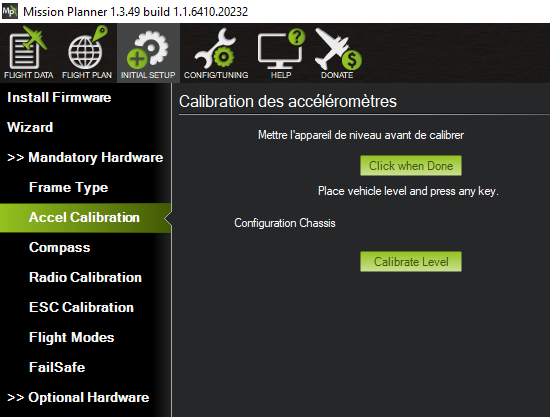
\includegraphics[width=7.5cm]{Images/A plat sur le ventre} & 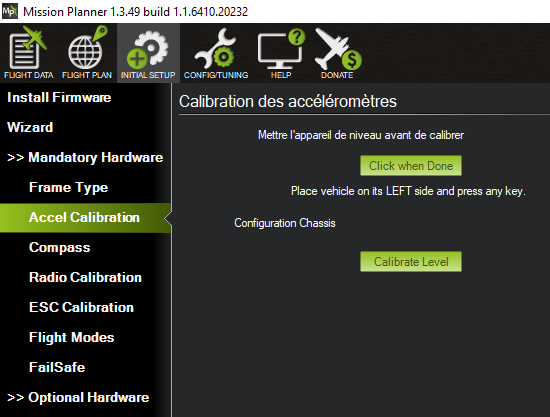
\includegraphics[width=7.5cm]{Images/Vertical sur son flanc gauche}\\
				\hline
				\centering
				
				1) A plat sur le ventre & 2) Vertical sur son flanc gauche \\
				
				\hline
				
				
				\centering
				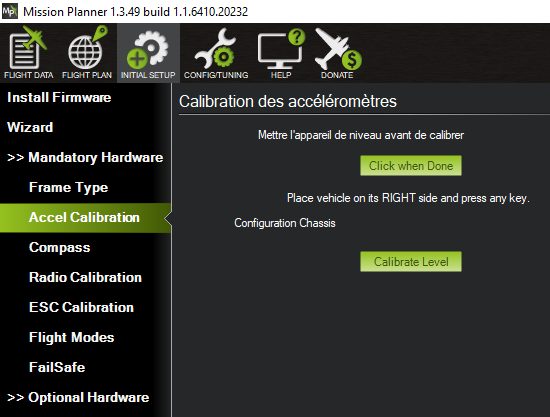
\includegraphics[width=7.5cm]{Images/Vertical sur son flanc droit} & 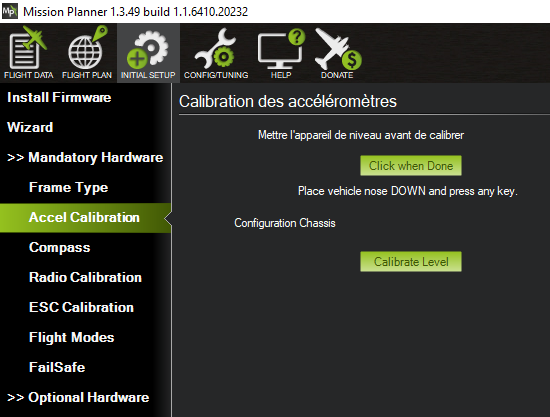
\includegraphics[width=7.5cm]{Images/Nez en bas}
				\\
				\hline
				
				
				\centering
				3) Vertical sur son flanc droit &   4) Nez en bas \\
				\hline
				
				
				\centering
				\includegraphics[width=7.5cm]{Images/Nez en l’air} & 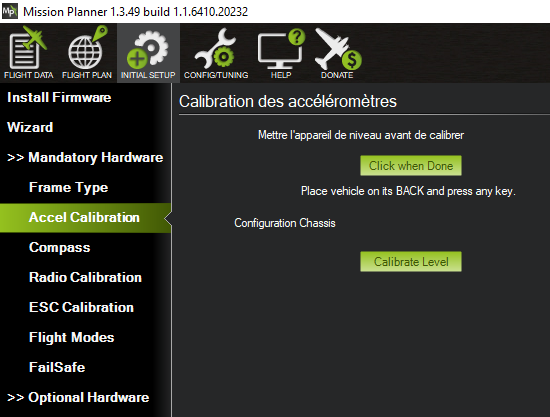
\includegraphics[width=7.5cm]{Images/Sur le dos}\\
				\hline
				\centering
				
				5) Nez en l’air &   6) Sur le dos \\
				\hline
			\end{tabular}
		\end{center}
	\end{table}	
	
	
	\newpage
	\subsection{Calibration du radio}
	Après s’être assuré que le récepteur est bien connecté au contrôleur de vol et qu’il est apparié à la
	radiocommande sous tension et correctement programmée, nous avons  accédé aux « Radio
	Calibration », cliqué sur le bouton « Calibrer Radio ». 
	Une fois validé, nous avons actionné toutes les commandes de la radio de leur minimum à leur maximum. 
	\begin{figure} [h]
		\begin{center}
			\centering
			\fbox{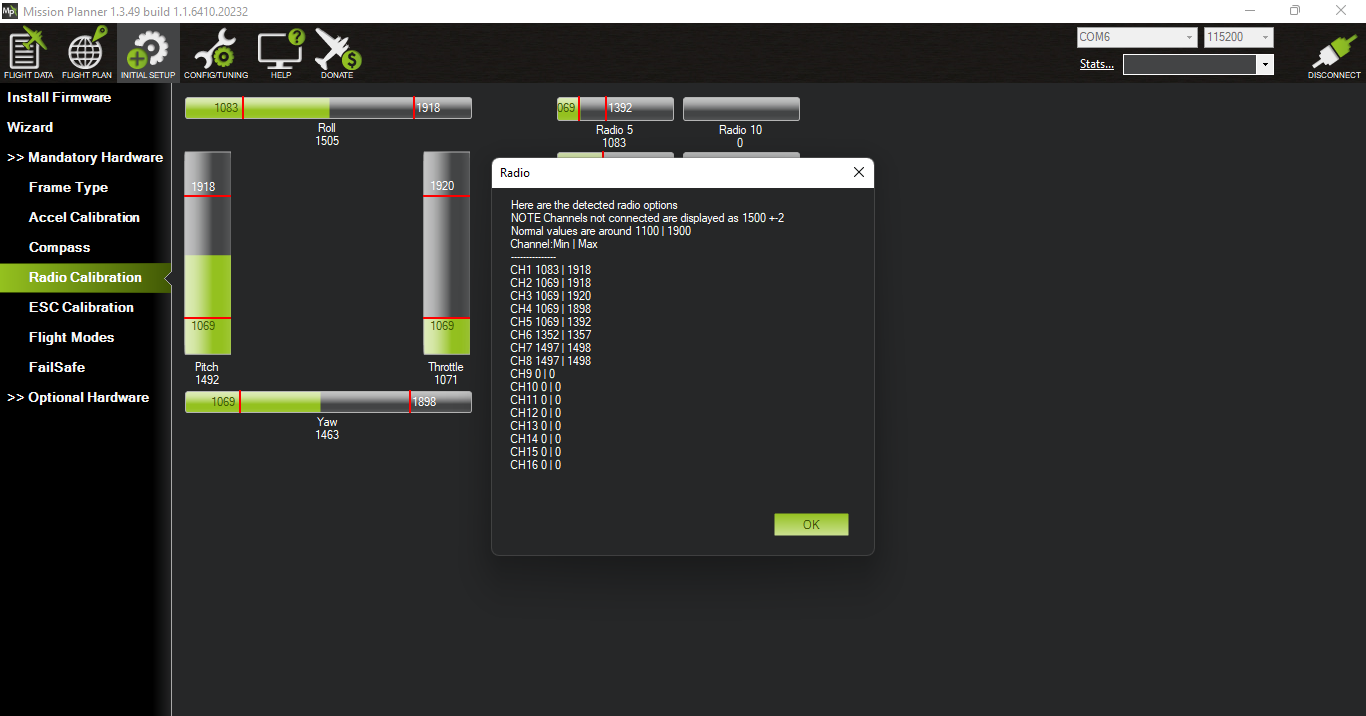
\includegraphics[width=0.8\linewidth]{Images/calibaration du radio}}
		\end{center}
		\caption{calibration du radio}
	\end{figure}
	
	\subsection{Configurations des modes de vol} 
	Notre APM 2.8 est caractérisé par la variété de ces modes de vol qui nous facilitent le pilotage et le contrôle de notre quadrirotor. Dans notre cas, nous avons utilisé deux modes de vol: le mode "Stabilize" nous permettant de contrôler notre drone manuellement et le mode "Alt Hold" permet le maitien de l'altitude constante. A savoir, le mode "Alt Hold" n'est pas applicable vu l'absence de GPS. Pour effectuer  cette configuration, nous avons accédé au <<Flight Modes>> comme le montre la figure ci-dessous.
	
	\begin{figure} [h]
		\begin{center}
			\centering
			\fbox{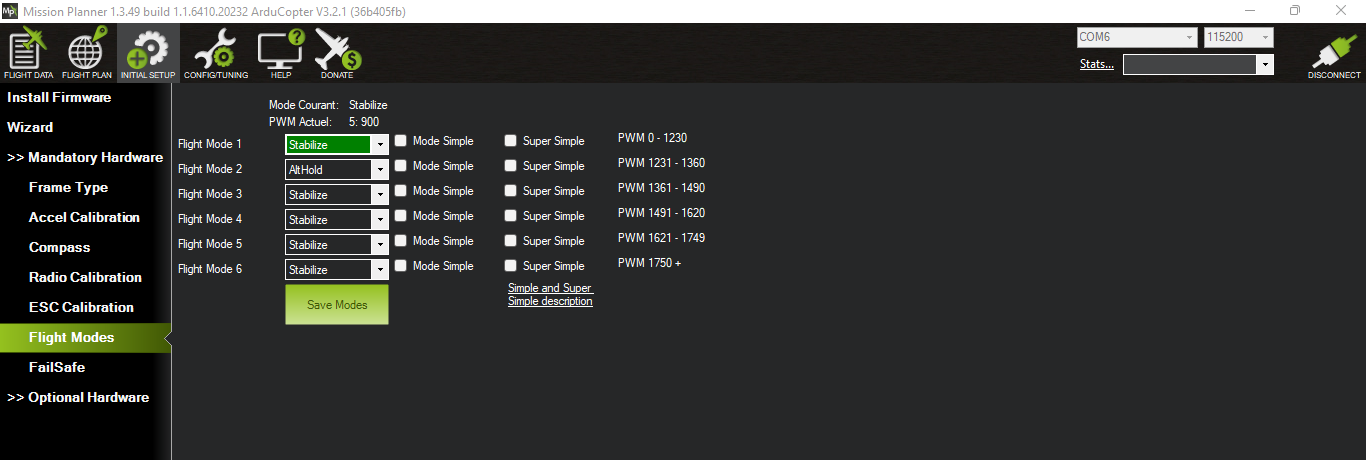
\includegraphics[width=0.8\linewidth]{Images/Modes de vol}}
		\end{center}
		\caption{Modes de vol}
	\end{figure}
	\newpage
	\subsection{Calibration des ESC}
	Les contrôleurs de vitesse doivent être étalonnés pour connaître les valeurs minimales et maximales du commande des Gaz. 
	
	
	La procédure d’étalonnage est la suivante. Nous avons en premier lieu coupé l’alimentation de l’appareil. Par la suite, nous avons allumé la radiocommande et positionné le manche des Gaz à son maximum. Ensuite, nous avons mis l’appareil sous tension en attendant que le contrôleur de vol démarre. Ainsi, nous avons coupé l’alimentation de l’appareil et nous l'avons remis sous tension. Après avoir entendu la mélodie issue des moteurs confirmant l’apprentissage de la valeur maximale des Gaz, nous avons baissé le manche des Gaz au minimum en attendant la mélodie de confirmation et actionner doucement les Gaz pour vérifier que tous les moteurs démarrent en même temps et tournent au même régime. Finalement, nous avons recoupé l’alimentation de l’appareil.
	\subsection{Configuration et calibration de la radiocommande}
	Concernant la configuration et la calibration de la radiocommande, nous avons passé par plusieurs étapes que nous expliquons ci-dessous. 
	\subsection{Mode de la radiocommande}
	Au début, notre radiocommande est activée en mode 1 où le bâton droite est relaché dans l'axe verticale et le bâton gauche est centré dans les deux axes. Afin de faciliter le pilotage de notre drone, nous avons activé notre radiocommande en mode 2  qui est l'inverse du mode précédent. Pour effectuer cette opération, nous avons tout d'abord retiré les six vis à l'arriére du boîtier. Ensuite, nous avons déplacé le ressort vers le bâton droite.  Finalement, nous avons fermé la radiocommande en remettant les vis.
	
	
	\subsubsection{SELECTION type de modèle}
	Cette fonctionnalité nous permet de sélectionner le type de modèles réduits d'avions qui seront utilisés ou affectés à un modèle particulier.
	Dans le menu Réglages Système, nous avons sélectionné SELE TYPE et appuyé sur MENU. Ensuite, en utilisant le haut ou bas nous avons choisi le type de modèle qui sera utilisé soit HELI, ACRO ou bien GLID. Après avoir sélectionné l'option Acro, nous avons appuyé sur MENU pour enregistrer, puis sur EXIT pour retourner au menu précédent.
	
	\begin{figure}[h]
		\begin{center}
			\centering
			\fbox{\includegraphics[width=0.6\linewidth]{Images/Type de modèle}}
		\end{center}
		\caption{type de modèle}
	\end{figure}
	\subsection{STICK SET }
	Dans le menu Réglages Système, nous avons sélectionné STICK SET, aprés avoir presser le MENU. Ensuite, nous avons choisi le mode le plus appropriée à notre style d'utilisation "modèle 2". Dés que cette étape est réalisé, nous avons effectué la sauvegarde de l'option sélectionnée en appuyant sur MENU. Aprés, nous avons appuyé sur le bouton EXIT pour revenir au menu précédent.
	\begin{figure}[h]
		\begin{center}
			\centering
			\fbox{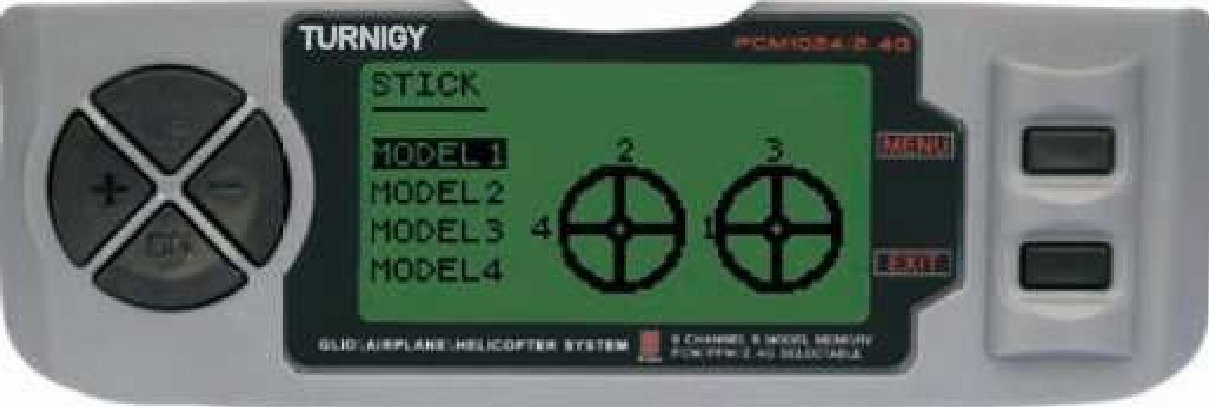
\includegraphics[width=0.6\linewidth]{Images/Les 4 modes}}
		\end{center}
		\caption{Les 4 modes}
	\end{figure}
	\newpage
	\begin{table}[h]
		\begin{center}
			\caption{Différentes Modes }
			\begin{tabular}{|c|c|}
				\hline
				
				\centering
				
				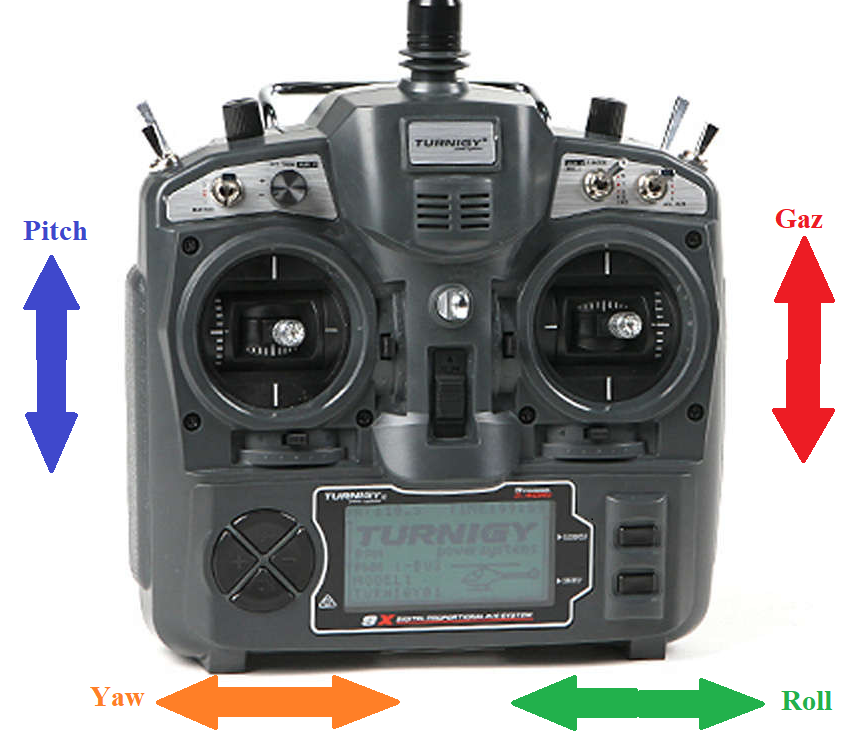
\includegraphics[width=4.8cm]{C:/Users/Ahmed Baha eddine/Downloads/Mode 1(Radiocommande)} & 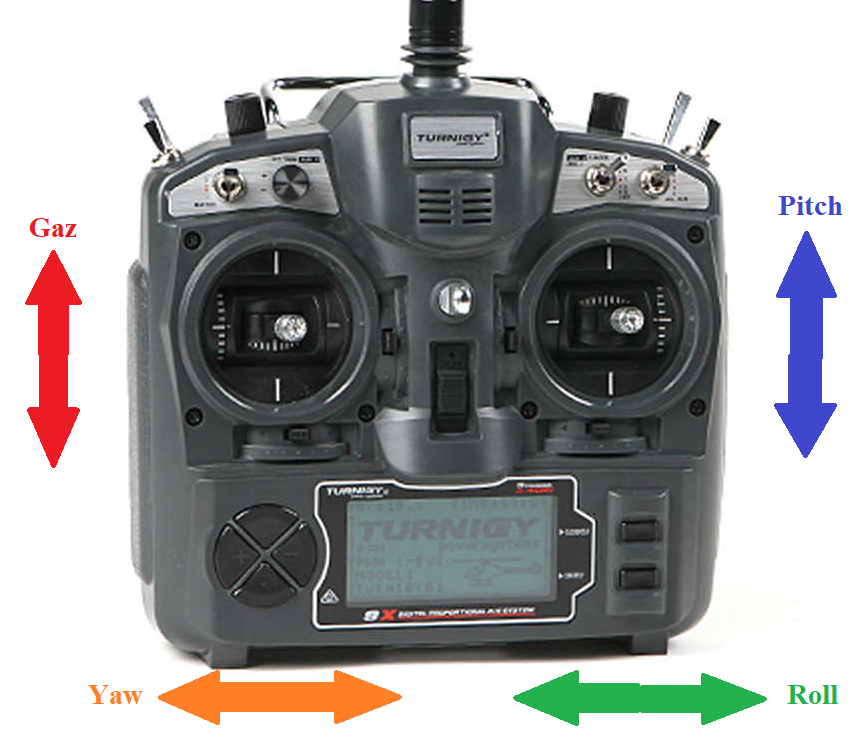
\includegraphics[width=4.8cm]{C:/Users/Ahmed Baha eddine/Downloads/Mode 2(Radiocommande)}\\
				\hline
				\centering
				
				Mode 1 & Mode 2 \\
				
				\hline
				\centering
				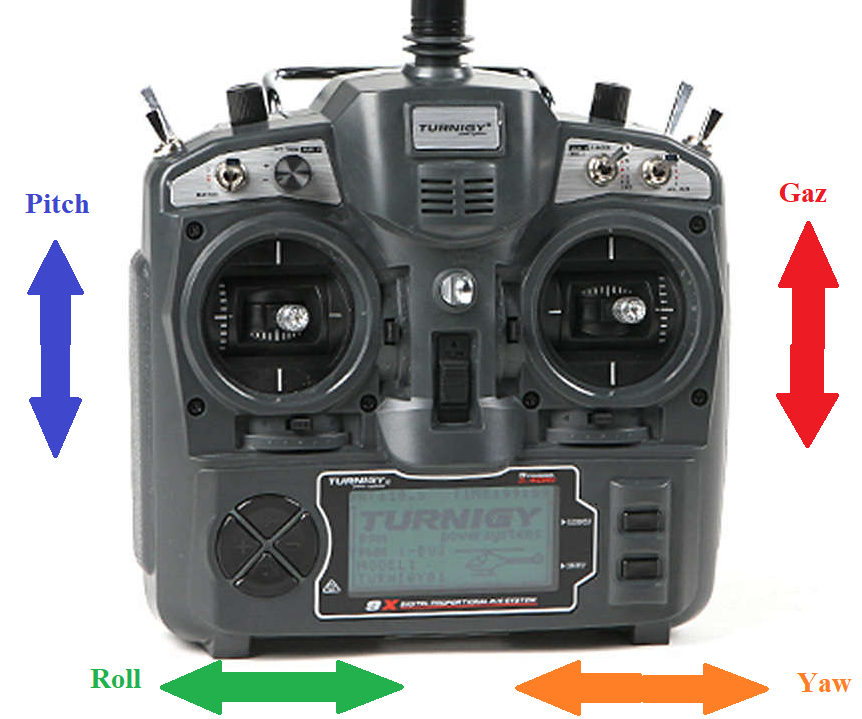
\includegraphics[width=4.69999cm]{C:/Users/Ahmed Baha eddine/Downloads/Mode 3(Radiocommande)}& 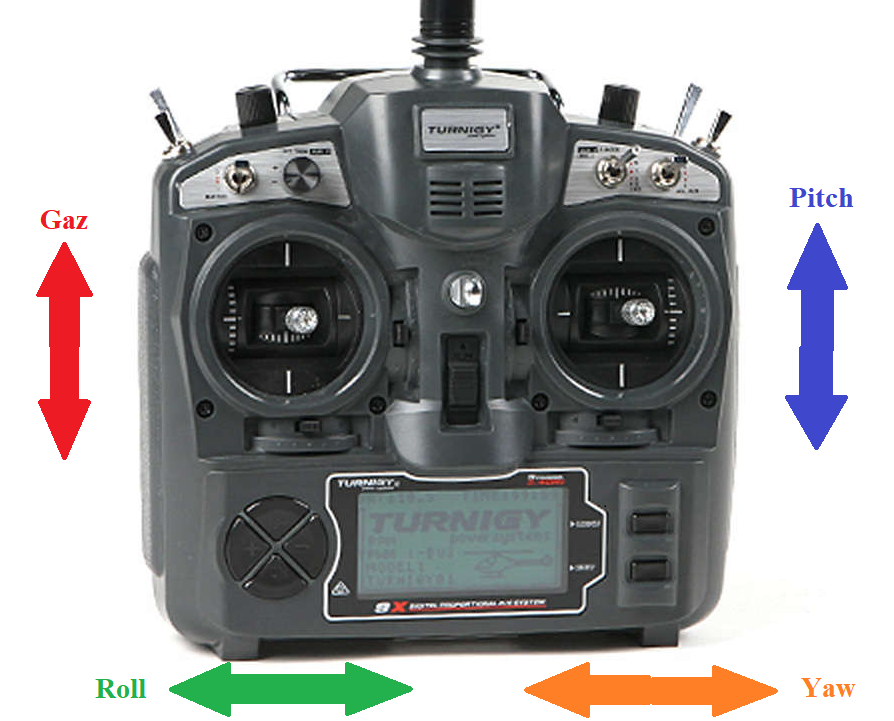
\includegraphics[width=4.69999cm]{C:/Users/Ahmed Baha eddine/Downloads/Mode 4(Radiocommande)}\\
				\hline
				\centering
				
				Mode 3 &  Mode 4 \\
				\hline
			\end{tabular}
		\end{center}
	\end{table}
	
	\subsection{ SELECT OSCILLANT TYPE}
	Cette fonctionnalité nous permet de sélectionner le type de modulation qui sera utilisé à un modèle particulier (PPM ou PCM).\\
	
	
	PPM: modulation de position d'impulsion (Pulse Modulation de position) 
	
	PCM: Pulse Code Modulation (Modulation d'impulsions codées).
	
	
	Dans le menu configuration système, nous avons cliqué sur Modeuat, appuyé sur MENU, sélectionné l'option désirée PPM et confirmé cette option sélectionnée en appuyant sur MENU. Ensuite, nous avons appuyé sur le bouton EXIT pour revenir au menu précédent.
	
	\begin{figure}[h]
		\begin{center}
			\centering
			\fbox{\includegraphics[width=0.6\linewidth]{Images/Sélection de mode pour HELI}}
		\end{center}
		\caption{Sélection de mode pour Acro}
	\end{figure}
	
	\subsection{Inversion des servos}
	La Servo Reverse nous permet de renverser le fonctionnement du servos afin de le manipuler conformément à nos besoin.
	
	
	
	Dans le MENU REGLAGES nous avons appuyé sur FUNC et sélectionné la fonction REVERSE en utilisant les touches haut ou bas. Ensuite, avec les touches + ou -
	nous avons appliqué cette fonction aux servos que nous avons affécté à cette opération. Aprés, nous avons appuyé sur MENU pour sauvegarder les nouveaux réglages et revenir au menu précédent.
	\begin{figure}[h]
		\begin{center}
			\centering
			\fbox{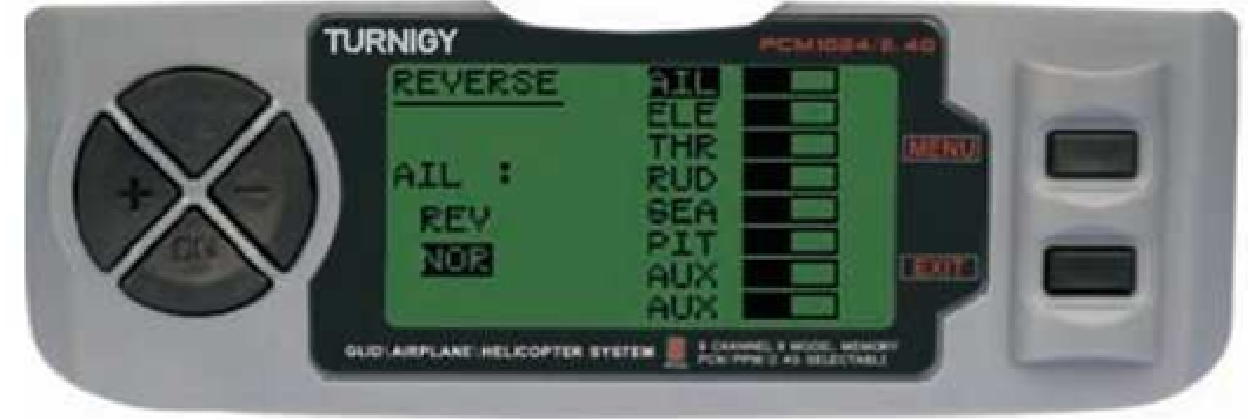
\includegraphics[width=0.6\linewidth]{Images/Inversion des servos}}
		\end{center}
		\caption{Inversion des servos}
	\end{figure}
	\section{Erreur eeprom}
	Lors de la configuration et du paramétrage de notre radiocommande, nous avons observé qu'elle s'éteind tout d'un coup et un message "erreur eeprom" s'affiche avec une alerte sonore. Nous avons effectué le redémarrage de la radiocommande mais en vain. Nous avons cherché comment résoudre ce problème et nous avons constaté qu'il faut la flasher. Pour effectuer cette opération, nous avons besoin d'un logiciel, d'un frimware à installer et d'un programmateur.
	\subsubsection{Microcontôleur Green-128}
	L'emmetteur de notre radiocommande turnigy 9x contient un microcontrôleur "Green-128" qui est compatible avec le microcontrôleur  "Atmega 128". Nous montrons dans la figure ci-dessous les pins de "Green-128". 
	\begin{figure}[h]
		\begin{center}
			\centering
			\fbox{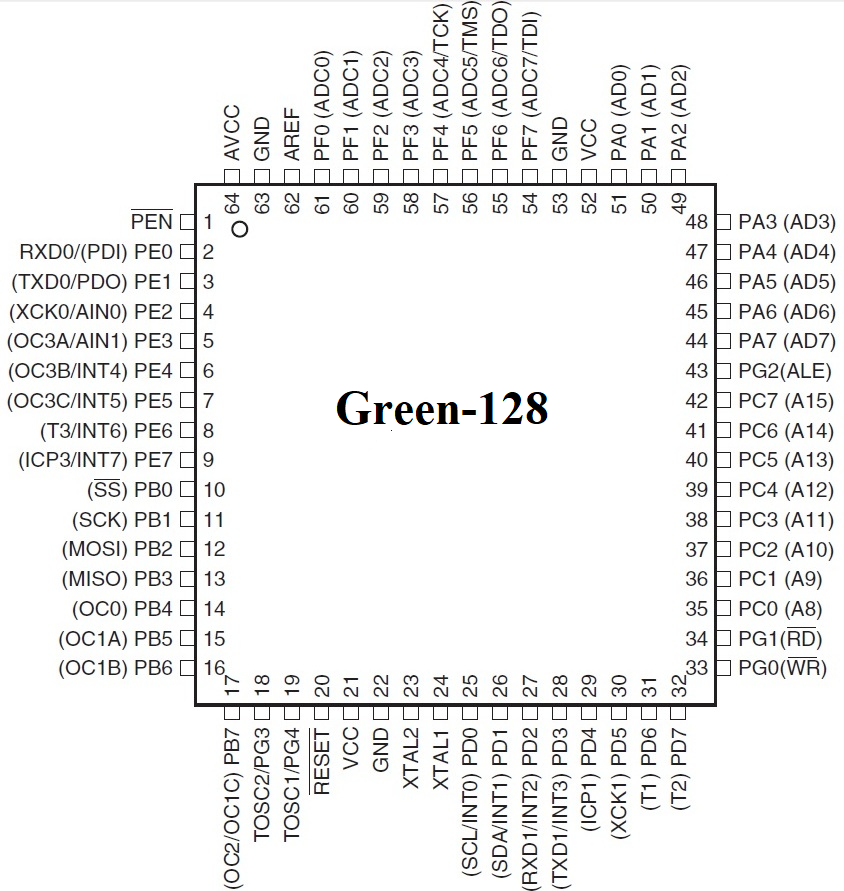
\includegraphics[width=0.6\linewidth]{C:/Users/Ahmed Baha eddine/Downloads/Green-128}}
		\end{center}
		\caption{IPins Green-128}
	\end{figure}
	\subsubsection{Programmateur Usbasp}
	Puisque le microcontrôleur "Green-128" est compatible avec "Atmega 128". Nous avons choisi le programmateur "Usbasp" vu qu'il est un programmateur pour la famille Atmel des microcôntroleurs. 
	
	\begin{figure}[h]
		\begin{center}
			\begin{minipage}{0.49\textwidth}
				\centering
				\hspace*{-1.5cm}\fbox{\includegraphics[width=0.6\linewidth]{C:/Users/Ahmed Baha eddine/Downloads/_p_r_pro-01-015-1}}
				\centering
				\hspace*{-1cm}\caption{Programmateur Usbasp}
				\label{fig:my_label}
			\end{minipage}
			\begin{minipage}{0.49\textwidth}
				\centering
				\fbox{\includegraphics[width=0.8\linewidth]{C:/Users/Ahmed Baha eddine/Downloads/usbasp-v2.0-idc-pinout}}
				\centering
				\hspace{1cm}\caption{Shéma pinout Usbasp}
				\label{fig:my_label}
			\end{minipage}
		\end{center}
	\end{figure}
	
	
	\subsubsection{Soudure des fils sur la radiocommande}
	Nous avons soudé 6 files de connexion  sur la carte de la radiocommande pour communiquer avec le programmateur Usbasp dans le but de téléverser le frimware.
	\begin{figure}[h]
		\begin{center}
			\centering
			\fbox{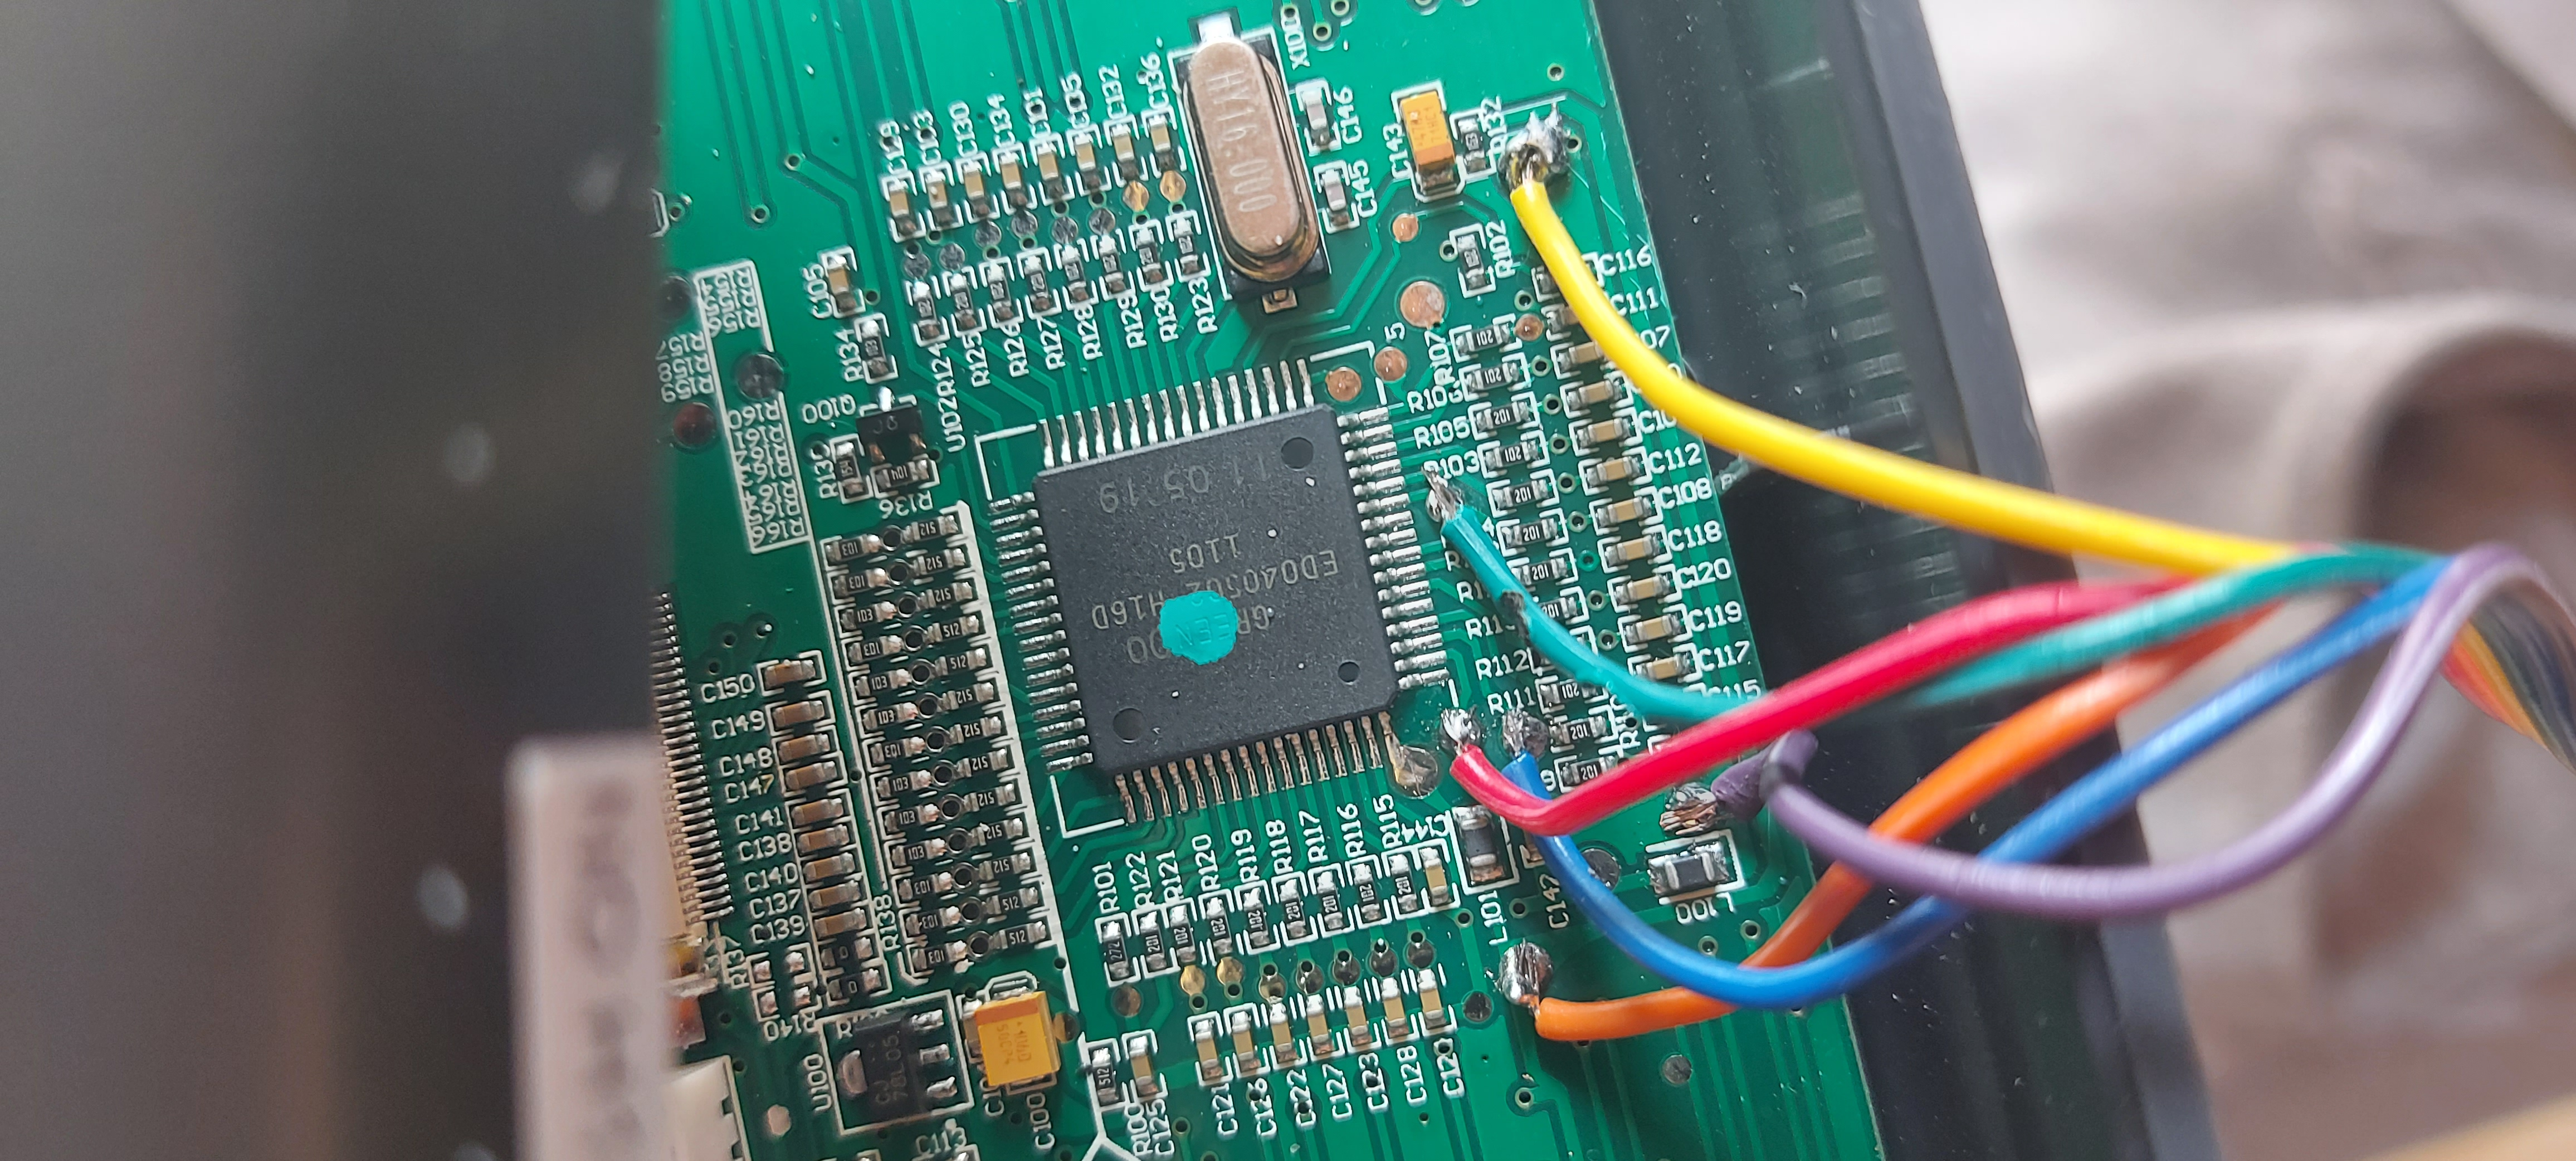
\includegraphics[width=0.8\linewidth]{Images/Soudure des files}}
		\end{center}
		\caption{Soudure des files}
	\end{figure}
	
	
	En se basant sur les figures 22,24 et 25, nous expliquons à travers ce tableau la communication entre le microcontrôleur "Green-128" et le programmateur "Usbasp" en spécifiant les couleurs attribuées à chaque connexion entre eux.
	
	\begin{table}[H]
		\begin{center}
			\caption{Communication entre le microcontrôleur green-128 et usbasp }
			\begin{tabular}{|c|c|c|}
				\hline
				\centering
				Green-128 &	Usbasp & couleur de file \\
				\hline
				PE0 pin 2 & Mosi pin 1 & Rouge  \\
				\hline
				PE1 pin 3 & Miso pin 9 & Blue  \\
				\hline
				PS1 (Sck)  pin 11 & Sck pin 7 & Vert  \\
				\hline
				Reset pin 20 & Reset pin 5 & Jaune \\
				\hline
				VCC pin 21 & VCC pin 2 &  ornge \\
				\hline
				GND pin 22 & GND pin 10 & violet \\
				\hline
			\end{tabular}
		\end{center}
	\end{table}
	\subsubsection{Frimware ER9X}
	Tout d'abord, nous avons téléchargé le frimware ER9X.hex et nous l'avons écrit dans la mémoire de la radiocommande à travers le logiciel "EEPE". Cette opération a été effectué avec succès, l'erreur eeprom n'existe plus et la radiocommande fonctionne avec ce frimware. Par la suite, lorsque nous avons essayé d'envoyer le signal de l'émetteur vers le récepteur, l'opération a échoué. Il faut donc installer le frimware original "AFHDS 2A".
	\subsubsection{Frimware AFHDS 2A}
	Après l'installation du Frimware AFHDS 2A, nous avons installé Companion9X et envoyé ce frimware vers la mémoire de la radiocommande. Nous avons réussi à envoyer les signaux au récepteur et notre radiocommande est reglée.
	\subsubsection{Conclusion}
	Dans ce chapitre, nous avons décrit l'environnement matériel et les différents logiciels que nous avons utilisé dans notre projet. En plus, nous avons présenté la réalisation de notre quadrirotor y compris son montage et la calibration des composants ainsi que l'erreur rencontrée dans notre travail.


